\documentclass[11pt,a4paper]{article}
\input{../../shared/preamble}
\SpeedHeader{Geometry}{5}

\begin{document}

\SpeedTitleBlock{Daily Geometry Drill \#5}{Henry Koduthore}
\SpeedMeta{Circles, arcs and tangency}{circle theorems, alternate segment, cyclic quadrilaterals, power of a point, tangent lengths, touching circles, circles in angles, segments and lenses}
\noindent\textit{New toolkit today: Angle at the centre $\cdot$ Cyclic quadrilaterals $\cdot$ Tangent $\perp$ radius $\cdot$ Power of a point $\cdot$ Touching circles: join the centres.}

\vspace{2pt}
\noindent\textit{Attempt each question before checking answers. Time yourself. No calculators. Diagrams are not to scale.}

\section*{Section A \quad Rapid Recognition \hfill{\normalfont\small($\leq$15 s each)}}
% ══════════════════════════════════════════════════════════════════════════════

\noindent\textit{Angle at the centre, angles on the same arc, cyclic opposite angles, the alternate segment, and power of a point. Know them cold.}

\begin{enumerate}

\item In a circle with centre $O$, the angle at the circumference subtending arc $AB$ is $20^\circ$. Write down the angle at the centre.

\item $AB$ is a diameter of a circle and $P$ is any other point on the circle. Write down $\angle APB$.

\item $ABCD$ is a cyclic quadrilateral with $\angle A=70^\circ$ and $\angle B=85^\circ$. Write down $\angle C$.

\item The tangent at $T$ to a circle makes an angle of $40^\circ$ with the chord $TA$. By the alternate segment theorem, write down the angle in the alternate segment subtended by $TA$.

\item Chords $AB$ and $CD$ of a circle intersect inside at $P$, with $PA=2$, $PB=6$ and $PC=3$. Write down $PD$.

\item A tangent from $P$ touches the circle at $T$, and a secant through $P$ cuts the circle at $A$ then $B$. Given $PT=3$ and $PA=1$, write down $PB$.

\item Write down the length of the tangent from $(7,0)$ to $x^2+y^2=36$.

\item Two tangents from the point $P$ to a circle of unknown radius make an angle of $60^\circ$ and $OP=6$. Write down the length of each tangent.

\item The two tangents from $P$ to the circle $x^2+y^2=25$ make an angle of $120^\circ$. Write down $OP$.

\item In the cyclic quadrilateral $ABCD$, $\angle BAC=30^\circ$. Write down $\angle BDC$.

\end{enumerate}

\section*{Section B \quad Manipulation Drills \hfill{\normalfont\small($\leq$50 s each)}}
% ══════════════════════════════════════════════════════════════════════════════

\noindent\textit{Draw the radius to the point of contact: it is perpendicular to the tangent. Then look for a right angle or a power of a point.}

\begin{enumerate}

\item A tangent at $T$ makes an angle of $55^\circ$ with chord $TA$. The angle in the alternate segment subtended by $TA$ is?
\begin{itemize}
\item[A)] $35^\circ$
\item[B)] $55^\circ$
\item[C)] $110^\circ$
\item[D)] $70^\circ$
\end{itemize}

\item $ABCD$ is cyclic with $\angle A=2x$ and $\angle C=3x$. Find $x$.
\begin{itemize}
\item[A)] $24$
\item[B)] $30$
\item[C)] $36$
\item[D)] $72$
\end{itemize}

\item A {\em tangential} (circumscribed) quadrilateral $ABCD$ has $AB=5$, $BC=7$ and $CD=6$. By Pitot's theorem ($AB+CD=BC+DA$), find $DA$.
\begin{itemize}
\item[A)] $4$
\item[B)] $6$
\item[C)] $8$
\item[D)] $18$
\end{itemize}

\item \begin{minipage}[t]{0.70\linewidth}
From external $P$, tangent $PT=12$ touches a circle and secant $PAB$ meets it with $PA=8$. Find the chord $AB$.
\begin{itemize}
\item[A)] $6$
\item[B)] $10$
\item[C)] $12$
\item[D)] $18$
\end{itemize}
\end{minipage}\hfill
\begin{minipage}[t]{0.26\linewidth}
\vspace{0pt}
\centering
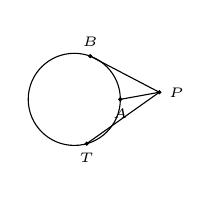
\begin{tikzpicture}[scale=0.45]
\draw (0,0) circle (1.3);
\draw (2.4,0.2) -- (1.3,0);
\draw (2.4,0.2) -- (0.45,1.22);
\draw[fill=black] (2.4,0.2) circle (1.2pt) node[right]{\tiny $P$};
\draw[fill=black] (1.3,0) circle (1.2pt) node[below]{\tiny $A$};
\draw[fill=black] (0.45,1.22) circle (1.2pt) node[above]{\tiny $B$};
\draw[fill=black] (0.35,-1.25) circle (1.2pt) node[below]{\tiny $T$};
\draw (2.4,0.2) -- (0.35,-1.25);
\end{tikzpicture}
\end{minipage}

\item From an external point $P$, two secants meet the same circle at $P$--$A$--$B$ and $P$--$C$--$D$, with $PA=4$, $PB=18$ and $PC=6$. Write down the length of the chord $CD$.

\item The point $P$ has $OP=6$ with respect to a circle of radius $3$. The angle between the two tangents from $P$ is?
\begin{itemize}
\item[A)] $30^\circ$
\item[B)] $45^\circ$
\item[C)] $60^\circ$
\item[D)] $90^\circ$
\end{itemize}

\item Two circles of radius $6$ each pass through the other's centre. They meet at $A$ and $B$. How long is $AB$? \textit{\small(after Primer 1.4 P16)}
\begin{itemize}
\item[A)] $6$
\item[B)] $12$
\item[C)] $6\sqrt2$
\item[D)] $6\sqrt3$
\item[E)] $3\sqrt3$
\end{itemize}

\item Two concentric circles have radii in the ratio $2:5$. $AC$ is a diameter of the larger circle, and the chord $BC$ of the larger circle touches the smaller circle. If $AB=8$, what is the radius of the larger circle? \textit{\small(after Primer 1.4 P13)}
\begin{itemize}
\item[A)] $16$
\item[B)] $20$
\item[C)] $8$
\item[D)] $12$
\item[E)] $10$
\end{itemize}

\item The line $ST$ is a chord of the larger of two concentric circles and touches the smaller one. If $ST=30$, find the area of the region between the circles. \textit{\small(after Primer 1.4 P8)}

\item $AB$ is a diameter of a circle and $C$ is a point on the circle with $\angle ABC=55^\circ$. Write down $\angle BAC$.

\end{enumerate}

\section*{Section C \quad Substitution \& Structure \hfill{\normalfont\small($\leq$90 s each)}}
% ══════════════════════════════════════════════════════════════════════════════

\noindent\textit{SMC Q18--22 level. Join the centres; tangent circles have centres $r_1+r_2$ apart and a common point on that line.}

\begin{enumerate}

\item \begin{minipage}[t]{0.60\linewidth}
$BC$ is a diameter of a circle and $CD$ is the tangent at $C$. The line $BD$ meets the circle again at $A$. If $AB=7$ and $AD=9$, what is the radius of the circle? \textit{\small(after Primer 1.4 P40)}
\begin{itemize}
\item[A)] $12$
\item[B)] $4\sqrt7$
\item[C)] $2\sqrt7$
\item[D)] $8$
\item[E)] $6$
\end{itemize}
\end{minipage}\hfill
\begin{minipage}[t]{0.36\linewidth}
\vspace{0pt}
\centering
\begin{tikzpicture}[scale=0.21]
\draw[speedgeom] (0,0) circle (5.29);
\draw[speedgeom] (0,5.29) -- (0,-5.29) -- (12,-5.29) -- cycle;
\draw (0,-4.6) -- (0.7,-4.6) -- (0.7,-5.29);
\node[above] at (0,5.29) {\small $B$}; \node[below] at (0,-5.29) {\small $C$};
\node[below] at (12,-5.29) {\small $D$}; \node[above right] at (5.25,0.66) {\small $A$};
\filldraw (5.25,0.66) circle (4pt);
\end{tikzpicture}
\end{minipage}

\item A regular octagon is inscribed in a circle of radius $2$, and $X$ is any point on the circle. What is the sum of the squares of the distances from $X$ to the eight vertices? \textit{\small(after SMC 2025 Q21)}
\begin{itemize}
\item[A)] $64$
\item[B)] $32$
\item[C)] $128$
\item[D)] $48$
\item[E)] $16$
\end{itemize}

\item \begin{minipage}[t]{0.60\linewidth}
Two circles of radius $2$ each pass through the other's centre. What is the area of the shaded region common to both circles? \textit{\small(after Primer 1.4 P24)}
\begin{itemize}[itemsep=3pt]
\item[A)] $\dfrac{4\pi}{3}-\sqrt3$
\item[B)] $\dfrac{8\pi}{3}-\sqrt3$
\item[C)] $\dfrac{4\pi}{3}+2\sqrt3$
\item[D)] $\dfrac{8\pi}{3}-2\sqrt3$
\item[E)] $2\pi-2\sqrt3$
\end{itemize}
\end{minipage}\hfill
\begin{minipage}[t]{0.36\linewidth}
\vspace{0pt}
\centering
\begin{tikzpicture}[scale=0.5]
\begin{scope}\clip (0,0) circle (2); \fill[gray!25] (2,0) circle (2); \end{scope}
\draw[speedgeom] (0,0) circle (2); \draw[speedgeom] (2,0) circle (2);
\filldraw (0,0) circle (1.5pt) (2,0) circle (1.5pt);
\end{tikzpicture}
\end{minipage}

\item \begin{minipage}[t]{0.60\linewidth}
A circle of radius $1$ touches both arms of a right angle. A larger circle touches both arms and the first circle. What is the radius of the larger circle? \textit{\small(after Primer 1.4 P35)}
\begin{itemize}
\item[A)] $1+\sqrt2$
\item[B)] $2+\sqrt2$
\item[C)] $2\sqrt2$
\item[D)] $3$
\item[E)] $3+2\sqrt2$
\end{itemize}
\end{minipage}\hfill
\begin{minipage}[t]{0.36\linewidth}
\vspace{0pt}
\centering
\begin{tikzpicture}[scale=0.27]
\draw[speedgeom] (0,12) -- (0,0) -- (12,0);
\draw[speedgeom] (1,1) circle (1); \draw[speedgeom] (5.83,5.83) circle (5.83);
\draw (0,0.5) -- (0.5,0.5) -- (0.5,0);
\end{tikzpicture}
\end{minipage}

\item \begin{minipage}[t]{0.60\linewidth}
Six equal discs lie between two concentric circles. Each disc touches its two neighbours and both circles. The inner circle has radius $1$. What is the radius of the outer circle? \textit{\small(after SMC 2016 Q21)}
\begin{itemize}
\item[A)] $3$
\item[B)] $2+\sqrt3$
\item[C)] $1+\sqrt3$
\item[D)] $2\sqrt3$
\item[E)] $4$
\end{itemize}
\end{minipage}\hfill
\begin{minipage}[t]{0.36\linewidth}
\vspace{0pt}
\centering
\begin{tikzpicture}[scale=0.33]
\draw[speedgeom] (0,0) circle (1); \draw[speedgeom] (0,0) circle (3);
\foreach \a in {0,60,...,300} \draw[speedgeom, fill=gray!20] (\a:2) circle (1);
\end{tikzpicture}
\end{minipage}

\item \begin{minipage}[t]{0.60\linewidth}
A circle of radius $1$ touches three sides of a $6\times2$ rectangle. A diagonal of the rectangle cuts the circle at $P$ and $Q$. What is the length $PQ$? \textit{\small(after SMC 2017 Q19)}
\begin{itemize}[itemsep=3pt]
\item[A)] $\dfrac{4\sqrt5}{5}$
\item[B)] $\dfrac{2\sqrt{15}}{5}$
\item[C)] $\sqrt3$
\item[D)] $\dfrac65$
\item[E)] $\dfrac{2\sqrt{10}}{5}$
\end{itemize}
\end{minipage}\hfill
\begin{minipage}[t]{0.36\linewidth}
\vspace{0pt}
\centering
\begin{tikzpicture}[scale=0.48]
\draw[speedgeom] (0,0) rectangle (6,2); \draw[speedgeom] (1,1) circle (1); \draw[speedgeom] (0,0) -- (6,2);
\filldraw (0.465,0.155) circle (1.5pt) (1.935,0.645) circle (1.5pt);
\node[above left] at (0.465,0.155) {\scriptsize $P$}; \node[below right] at (1.935,0.645) {\scriptsize $Q$};
\end{tikzpicture}
\end{minipage}

\item \begin{minipage}[t]{0.60\linewidth}
An isosceles trapezium has parallel sides of lengths $8$ and $18$, and all four of its sides touch a circle. What is the radius of the circle? \textit{\small(after SMC 2012 Q20)}
\begin{itemize}[itemsep=3pt]
\item[A)] $\dfrac{13}{2}$
\item[B)] $5$
\item[C)] $12$
\item[D)] $6$
\item[E)] $4\sqrt3$
\end{itemize}
\end{minipage}\hfill
\begin{minipage}[t]{0.36\linewidth}
\vspace{0pt}
\centering
\begin{tikzpicture}[scale=0.15]
\draw[speedgeom] (0,0) -- (18,0) -- (13,12) -- (5,12) -- cycle;
\draw[speedgeom] (9,6) circle (6);
\node[below] at (9,0) {\scriptsize $18$}; \node[above] at (9,12) {\scriptsize $8$};
\end{tikzpicture}
\end{minipage}

\item \begin{minipage}[t]{0.60\linewidth}
$ABCD$ is a cyclic quadrilateral in which $AB$ is a diameter of the circle, $AB=25$ and $AD=BC=15$. What is the length $CD$? \textit{\small(after Primer 1.4 P33)}
\begin{itemize}
\item[A)] $10$
\item[B)] $15$
\item[C)] $13$
\item[D)] $9$
\item[E)] $7$
\end{itemize}
\end{minipage}\hfill
\begin{minipage}[t]{0.36\linewidth}
\vspace{0pt}
\centering
\begin{tikzpicture}[scale=0.12]
\draw[speedgeom] (0,0) circle (12.5);
\draw[speedgeom] (-12.5,0) -- (12.5,0) -- (3.5,12) -- (-3.5,12) -- cycle;
\node[left] at (-12.5,0) {\small $A$}; \node[right] at (12.5,0) {\small $B$};
\node[above right] at (3.5,12) {\small $C$}; \node[above left] at (-3.5,12) {\small $D$};
\end{tikzpicture}
\end{minipage}

\end{enumerate}

\section*{Section D \quad Challenge \hfill{\normalfont\small(SMC Q23--25 / BMO1 difficulty)}}
% ══════════════════════════════════════════════════════════════════════════════

\noindent\textit{Coordinates, the sine rule or a chain of similar figures. Diagrams are not to scale.}

\begin{enumerate}

\item \begin{minipage}[t]{0.60\linewidth}
Three circles each touch both arms $QP$ and $QR$ of an angle, and each touches the next. The largest radius is $4$ times the smallest. What is $\cos\angle PQR$? \textit{\small(after SMC 2011 Q24)}
\begin{itemize}[itemsep=3pt]
\item[A)] $\dfrac79$
\item[B)] $\dfrac13$
\item[C)] $\dfrac23$
\item[D)] $\dfrac89$
\item[E)] $\dfrac{4\sqrt2}{9}$
\end{itemize}
\end{minipage}\hfill
\begin{minipage}[t]{0.36\linewidth}
\vspace{0pt}
\centering
\begin{tikzpicture}[scale=0.19]
\draw[speedgeom] (0,0) -- (17,6.01); \draw[speedgeom] (0,0) -- (17,-6.01);
\draw[speedgeom] (3,0) circle (1); \draw[speedgeom] (6,0) circle (2); \draw[speedgeom] (12,0) circle (4);
\node[left] at (0,0) {\small $Q$}; \node[above] at (17,6.01) {\small $P$}; \node[below] at (17,-6.01) {\small $R$};
\end{tikzpicture}
\end{minipage}

\item \begin{minipage}[t]{0.60\linewidth}
$OAB$ is a quarter circle with radius $4$. A semicircle is drawn on $OA$ as diameter, inside the quarter circle. A circle touches $OB$, the semicircle and the arc $AB$. What is its radius? \textit{\small(after SMC 2014 Q19)}
\begin{itemize}[itemsep=3pt]
\item[A)] $\dfrac43$
\item[B)] $1$
\item[C)] $\dfrac23$
\item[D)] $\sqrt2$
\item[E)] $\dfrac34$
\end{itemize}
\end{minipage}\hfill
\begin{minipage}[t]{0.36\linewidth}
\vspace{0pt}
\centering
\begin{tikzpicture}[scale=0.55]
\draw[speedgeom] (0,4) -- (0,0) -- (4,0); \draw[speedgeom] (4,0) arc (0:90:4);
\draw[speedgeom] (4,0) arc (0:180:2); \draw[speedgeom, fill=gray!20] (1,2.828) circle (1);
\node[below left] at (0,0) {\small $O$}; \node[below] at (4,0) {\small $A$}; \node[left] at (0,4) {\small $B$};
\end{tikzpicture}
\end{minipage}

\item A triangle with angles $30^\circ$, $45^\circ$ and $105^\circ$ is inscribed in a circle of radius $2$. What is its area? \textit{\small(after SMC 2021 Q22)}
\begin{itemize}
\item[A)] $2+\sqrt3$
\item[B)] $2\sqrt3$
\item[C)] $1+\sqrt3$
\item[D)] $3+\sqrt3$
\item[E)] $2$
\end{itemize}

\item \begin{minipage}[t]{0.60\linewidth}
Two circles of radius $5$ have centres $2$ apart. A square is inscribed in the region common to both circles, with its sides parallel and perpendicular to the line of centres. What is the area of the square? \textit{\small(after SMC 2019 Q25)}
\begin{itemize}
\item[A)] $64$
\item[B)] $32$
\item[C)] $25$
\item[D)] $36$
\item[E)] $48$
\end{itemize}
\end{minipage}\hfill
\begin{minipage}[t]{0.36\linewidth}
\vspace{0pt}
\centering
\begin{tikzpicture}[scale=0.24]
\begin{scope}\clip (-1,0) circle (5); \fill[gray!12] (1,0) circle (5); \end{scope}
\draw[speedgeom] (-1,0) circle (5); \draw[speedgeom] (1,0) circle (5);
\draw[speedgeom, fill=gray!35] (-3,-3) rectangle (3,3);
\filldraw (-1,0) circle (3pt) (1,0) circle (3pt);
\end{tikzpicture}
\end{minipage}

\item \begin{minipage}[t]{0.60\linewidth}
$ABCD$ is a cyclic quadrilateral whose diagonals are perpendicular and meet at $E$. The line through $E$ perpendicular to $AB$ meets $CD$ at $F$. Prove that $F$ is the midpoint of $CD$.
\end{minipage}\hfill
\begin{minipage}[t]{0.36\linewidth}
\vspace{0pt}
\centering
\begin{tikzpicture}[scale=0.42]
\draw[speedgeom] (1,-1) circle (3.162);
\draw[speedgeom] (4,0) -- (0,2) -- (-2,0) -- (0,-4) -- cycle;
\draw[speedaux] (4,0) -- (-2,0) (0,2) -- (0,-4);
\draw[speedgeom] (0.8,1.6) -- (-1,-2);
\node[right] at (4,0) {\small $A$}; \node[above] at (0,2) {\small $B$}; \node[left] at (-2,0) {\small $C$};
\node[below] at (0,-4) {\small $D$}; \node[above left] at (0,0) {\scriptsize $E$}; \node[left] at (-1,-2) {\small $F$};
\end{tikzpicture}
\end{minipage}

\end{enumerate}

\SpeedClosing{``With circles, draw what you cannot see: the centres, the radii to the points of contact, and the line joining two centres.''}

\end{document}
